\chapter{Question4}
\section{问题概述}
%
%%对问题的直观描述
%
本问题要求利用神经网络实现语言识别功能。

%
%对项目已有代码的阅读和理解
%

%
%解决问题的思路和想法
%

\section{算法设计}
%
%用自己的语言描述解决问题所使用的算法的原理及功能,设计思路和算法流程图
%
项目要求使用RNN解决该问题。它的核心思想是,对于输入的单词,以字母为单位不断更新预测的结果,并且
除了当前的字母外,还以上一次的得出的结果作为输入(除首字母外)。这要求我们构造两个函数$f_{init}$和$f_{mid}$
来分别处理首字母和后续字母的情形。

由于不排除只由一个字母组成的单词的可能,所以$f_{init}$的输出大小也必须符合最终结果的要求,特别地,大小必须相同。

由于$f_{init}$的作用只占一小部分,所以可以直接沿用之前的神经网络结构,即两层线性层加上一层非线性层。

对于$f_{mid}$,首先要处理的是将上一层得到的输出和当前的输入结合在一起。为此,我先对当前输入和上一层的输出分别使用一层线性层,
以统一它们的形状,然后使用逐元素的矩阵加法将它们合并在一起,以方便后续神经网络的搭建。最终,我在此基础之上又添加了两层隐藏层。

具体神经网络架构如下图所示,其中last指模型在上一个输入中得到的结果,线性层中均包含了偏置值,非线性层均使用ReLU函数。

\begin{figure}[!h]
\centering    
\begin{forest}
    for tree={
      grow=west,
      edge={<-},
      parent anchor=west,
      child anchor=east,
      align=center,
      anchor=east,
      calign=center,
      calign primary angle=60,
      calign secondary angle=60,
      s sep=10mm,
      l sep=5mm,
      edge+={thick, color=black},
    }
    [
        输出
        [
            线性层
            [
                非线性层
                [
                    线性层
                    [
                        非线性层
                        [+
                        [
                            线性层
                            [last]
                        ]
                        [线性层
                        [输入]
                        ]
                        ]
                    ]
                ]
            ]    
        ]
    ]
  \end{forest}
  \caption{神经网络架构}
\end{figure}


训练是否结束的依据仍然是在验证集上得到的准确率。
\section{算法实现}
%
%在算法原理的基础上,结合代码,讲述算法的实现细节、核心函数、模块输入输出,数据结构定义等内容
%
%
为了避免学习率设置不当而导致训练后期出现梯度消失或梯度爆炸的问题,我让学习率以已训练批次的对数的倒数的速率递减。
\begin{lstlisting}[emph={[3]dataset,x,y,xs},emphstyle={[3]\color{vscode_parametercolor}},emph={[4]LanguageIDModel,DigitClassificationModel,RegressionModel,GameState,MinimaxAgent,AlphaBetaAgent},emphstyle={[4]\color{vscode_classcolor}}]
class LanguageIDModel(object):
    def __init__(self):
        self.num_chars = 47
        self.languages = ["English", "Spanish", "Finnish", "Dutch", "Polish"]
        self.layer_size = 1<<9
        self.second_layer_size = 1<<9
        self.feature_num = self.num_chars
        self.output_num = len(self.languages)
        self.learning_rate = 0.1
        self.batch_size = 200
        self.threshold = 0.87
        self.cnt = 1

        self.w1 = nn.Parameter(self.feature_num,self.layer_size)
        self.b1 = nn.Parameter(1,self.layer_size)
        self.w2 = nn.Parameter(self.layer_size,self.second_layer_size)
        self.b2 = nn.Parameter(1,self.second_layer_size)
        self.w3 = nn.Parameter(self.second_layer_size,self.output_num)
        self.b3 = nn.Parameter(1,self.output_num)
        self.w4 = nn.Parameter(self.layer_size,self.output_num)
        self.b4 = nn.Parameter(1,self.output_num)
        self.w_hidden = nn.Parameter(self.output_num,self.layer_size)
        self.W = [self.w1,self.b1,self.w2,self.b2,self.w_hidden,self.w3,self.b3,self.w4,self.b4]

    def init(self,x0):
        return nn.AddBias( nn.Linear( nn.ReLU( nn.AddBias( nn.Linear(x0,self.w1),self.b1)),self.w4),self.b4)

    def mid(self,h,x):
        return \
            nn.AddBias( nn.Linear(
        nn.ReLU(
                    nn.AddBias( nn.Linear(
                        nn.ReLU(
                                    nn.Add( nn.AddBias( nn.Linear(x,self.w1),self.b1),nn.Linear(h,self.w_hidden))
                                ),
                    self.w2),self.b2)
                ),
            self.w3),self.b3)

    def run(self, xs):
        last = None
        for i,x in enumerate(xs):
            if not i:
                last = self.init(x)
            else:
                last = self.mid(last,x)
        return last

    def get_loss(self, xs, y):
        return nn.SoftmaxLoss(self.run(xs),y)

    def train(self, dataset):
        for x,y in dataset.iterate_forever(self.batch_size):
            self.cnt += 1
            gradients = nn.gradients(self.get_loss(x,y),self.W)
            for i,w in enumerate(self.W):
                w.update(gradients[i],-self.learning_rate*(1/log(self.cnt)))
            if dataset.get_validation_accuracy() >= self.threshold:
                break
\end{lstlisting}
\section{实验结果}
我成功获得了本问题的所有分数。本文的评分标准是模型在测试集上的准确率达到81\%及以上。
\begin{figure}[htbp]
    \centering
    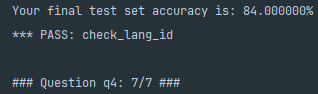
\includegraphics{pic/q4.png}
    \caption{Question4实验结果}\label{q4}
\end{figure}
%
%实验中遇到的问题及解决方案,收获和思考:对算法的理解、优缺点的评价、算法的适用场景
%
